%------------------------------%
%------------------------------%
\chapter{chapitre3}
\markboth{chapitre3}{chapitre3}
%------------------------------%
%------------------------------%
Voir figure \ref{fig:mafigure3}.


\begin{figure}[htbp]
   \begin{center}
      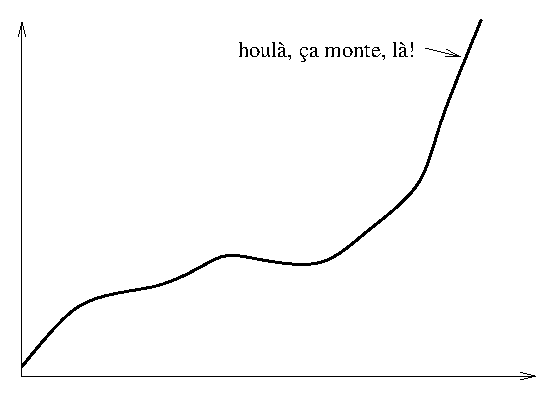
\includegraphics[width=0.8\linewidth]{chapitre3/fig/mafigure.eps}
   \end{center}
   \caption[ titre court]
   {\footnotesize Titre plus long avec des explications.}
   \label{fig:mafigure3}
\end{figure}
